\documentclass[a4paper, 12pt]{article}
\usepackage[utf8]{inputenc}  % Unicode
\usepackage[french]{babel}
\usepackage{geometry}
\usepackage{graphics}
\usepackage[pdftex]{graphicx, color}
\usepackage{pdfpages}
\DeclareGraphicsExtensions{.jpg,.png}
\pdfoutput=1
\usepackage[pdftex,
	bookmarks = true,           % Signets
	bookmarksnumbered = true,   % Signets numerotes
	pdfstartview = FitV,        % La page prend toute la hauteur
	colorlinks=true,
	citecolor=black,urlcolor=blue,linkcolor=black,
	pdfauthor={Auteur},
	pdftitle={Titre},
 	pdfsubject={Sujet},
%	pdfkeywords={},	% Besoin de keywords ?
	plainpages=false,
	pdfpagelabels,
	breaklinks=true,
   	hyperindex,
	linktocpage=true	% pour colorier seulement le numéros dans la TOC	
]{hyperref}
\usepackage{float}
\usepackage{listings}

\newcommand{\HRule}{\rule{\linewidth}{0.5mm}}

\newcommand*\styleC{\fontsize{9}{10pt}\selectfont }
\newcommand*\styleD{\fontsize{9}{10pt}\usefont{OT1}{pag}{m}{n}\selectfont }

\makeatletter
% on fixe le langage utilisé
\lstset{language=matlab}
\edef\Motscle{emph={\lst@keywords}}
\expandafter\lstset\expandafter{%
  \Motscle}
\makeatother


\definecolor{Ggris}{rgb}{0.45,0.48,0.45}

\lstset{emphstyle=\ttfamily\color{blue}, % les mots réservés de matlab en bleu
basicstyle=\ttfamily\styleC, % 
keywordstyle=\ttfamily,
commentstyle=\color{Ggris}\styleD, % \styleD commentaire en gris
numberstyle=\tiny\color{black},
numbers=left,
numbersep=10pt,
lineskip=0.7pt,
showstringspaces=false}
%  % inclure le fichier source
\newcommand{\FSource}[1]{%
\lstinputlisting[texcl=true]{#1}
}

%%%%%%%%%
\textwidth=15cm
\textheight=21cm
%\hoffset=-2.5cm
\tolerance=9000
\hbadness=9000
\pretolerance=2500





\begin{document}
%\rmfamily

\begin{titlepage}
\begin{center}



\textsc{\Large Rapport de TP - SY26}\\[0.5cm]
\vspace{4cm}
% Title
\HRule \\[0.4cm]
{ \huge \bfseries TP02 - Codage de Huffman \\[0.4cm] }

\HRule \\[1.5cm]

% Author and supervisor
\begin{minipage}{0.4\textwidth}
\begin{flushleft} \large
R\'emi \textsc{Burtin}
\end{flushleft}
\end{minipage}
\begin{minipage}{0.4\textwidth}
\begin{flushright} \large
Cyril \textsc{Fougeray}
\end{flushright}
\end{minipage}

\vspace{4cm}

{\large \today}



\vfill
% Bottom

\includegraphics[width=0.25\textwidth]{logo.jpg}\\[0.5cm]

\textsc{\LARGE Universit\'{e} de Technologie de Compi\`{e}gne}\\[1.5cm]


\end{center}
\end{titlepage}


%\begin{abstract} 
%\end{abstract} 

%{\bf Keywords:} \newline


\clearpage

\section{Introduction}
L'objectif de ce TP est de comparer le codage de Huffman au codage arithmétique. Pour cela, nous travaillons sur une image ('lena.bmp') en niveaux de gris, ce qui permet de fixer une seule valeur (entre 0 et 255) pour chaque pixel de l'image. Nous avons donc réalisé deux scripts, chacun codant et décodant une image en utilisant un des deux algorithmes.

\section{Codeur de Huffman}

\subsection{Mise en oeuvre}

L'image que nous manipulons pour réaliser l'encodage/décodage selon Huffman ne contient qu'une seule composante correspondant à l'intensité du gris, à la différence d'une image couleur comportant 3 composantes (rouge, vert, bleu). L'image originale étant en couleurs, nous la convertissons en utilisant la fonction \textit{rgb2gray} qui retourne une matrice à deux dimensions, de même taille que l'image.\\

Afin de réaliser l'encodage, il est nécessaire de connaître la loi de probabilités des niveaux de gris de l'image. Pour cela, nous commençons par réaliser l'histogramme comptant le nombre d'occurrences (l'effectif) de chaque valeur de gris. L'histogramme est en fait un vecteur de taille 256, ce qui correspond aux différentes valeurs de gris. Ainsi, à l'index $x\in[1, 256]$, nous obtenons le nombre d’occurrences de l'intensité de gris égale à $(x-1)$ dans l'image (le gris est codé sur un octet, donc sa valeur est comprise entre 0 et 255). Afin d'obtenir une fonction densité de probabilités ($\sum P(X=x_{i}) = 1$), nous normalisons l'histogramme en divisant chacune de ses valeurs par le nombre total de pixels dans l'image. \\ 

\begin{figure}[H]
\begin{center}
	 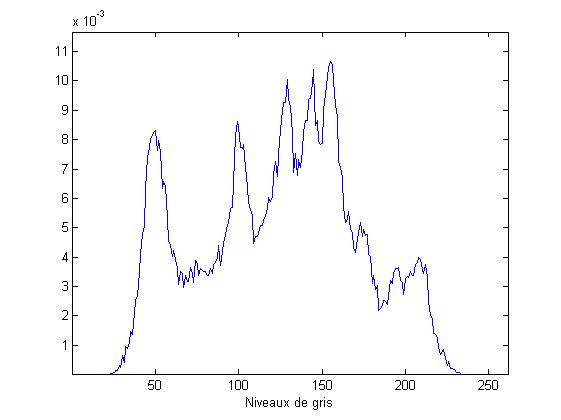
\includegraphics[scale=0.6]{../proba.jpg}
	 \caption{\label{probaGris} Densité de probabilités, niveaux de gris dans l'image \textit{lena.bmp}}
\end{center}
\end{figure}

L'algorithme d'Huffman fonctionne de sorte que les symboles ayant la plus grande probabilité utilisent le moins de ressources afin d'utiliser le moins de bande passante possible, et vice-versa, afin d'améliorer la compression. Dans le cas de notre image, beaucoup d'intensités de gris n'apparaissent pas dans l'image (leur probabilité d'apparition est alors nulle) : elles correspondent aux indexes de l'histogramme ayant pour valeur 0 (\textit{cf. figure \ref{probaGris}}). Afin de ne pas encoder ces valeurs qui prendraient beaucoup de ressources inutilement, il faut supprimer ces valeurs et créer un nouvel histogramme ayant des valeurs toutes strictement positives. Afin de reconstruire l'image originale après encodage/décodage, nous devons alors établir une table de correspondance. Ainsi, chaque index de l'histogramme sans zéro devra être lié à sa valeur de gris présent dans l'image. \\

Selon la longueur de l'histogramme sans zéro, nous créons un dictionnaire avec les nouveaux symboles allant de 0 à L, L étant la taille du nouvel histogramme. Dans le tableau~\ref{tab:Histogrammes} page~\pageref{tab:Histogrammes}, nous ne conservons que les niveaux de gris présents dans l'image, nous voyons que l'index dans le nouvel histogramme ne correspond plus au niveaux de gris. Une table de correspondance est alors créée, \textit{cf. tableau \ref{tab:TableDeCorrespondance}}. \\

\begin{table}[!h]
	\centering
		\begin{tabular}{|c c|c c c|}
			\hline 
			\multicolumn{2}{|c|}{Histogramme simple} & \multicolumn{3}{|c|}{ Histogramme sans zéros } \\
			\hline Index & Effectif & Index & Effectif & Niveau de gris\\
			\hline
						1 & 0 & 1  & 2 & 3 \\
						2 & 0 & 2  & 6 & 5\\
						3 & 2 & 3  & 7 & 6\\
						4 & 0 &  & &  \\
						5 & 6 &  & &  \\
						6 & 7 &  & &  \\
						7 & 0 &  & & 	\\
						8 & 0 &  & & 	\\
			\hline
		\end{tabular}
	\caption{Exemple - Histogrammes}
	\label{tab:Histogrammes}
\end{table}

L'index de l'histogramme sans zéro correspond à un symbole lors de la création du dictionnaire par la fonction \textit{huffmandict}. \\

\begin{table}[!h]
	\centering
		\begin{tabular}{|c|c|}
			\hline 
				Index (Histogramme sans zéro) & Niveau de gris associé \\
			\hline 
				1 & 3 \\
				2 & 5 \\
				3 & 6 \\
			\hline
		\end{tabular} \\
	\caption{Exemple - Table de correspondance}
	\label{tab:TableDeCorrespondance}
\end{table}

Une fois le dictionnaire créé, nous devons adapter les niveaux de gris présents dans l'image pour qu'ils correspondent aux symboles passées lors de l'encodage. Pour cela, nous utilisons la table de correspondance. En suivant l'exemple ci-dessus, nous voyons que les pixels de niveau de gris 3 doivent être remplacés par 1. \\

Nous encodons maintenant l'image via la fonction \textit{huffmanenco}. La fonction reçoit l'image dans un vecteur ligne ainsi que le dictionnaire comprenant la valeur d'encodage de chaque symbole. Elle nous retourne l'image encodé (soit une image compressée). \\

Nous décodons ensuite afin de retrouver l'image originale. La fonction \textit{huffmandeco} permet de retrouver le vecteur ligne correspondant à l'image originale. Comme nous l'avons vu, et d'après l'exemple, une valeur décodée égale à 1 correspond à un niveau de gris de 3. Nous devons alors faire la conversion de chacune des valeurs du vecteur ligne vers sa valeur de gris associée. Ensuite, nous reconstruisons l'image à partir du vecteur colonne vers une matrice 2D, grâce à la fonction \textit{reshape}. L'image peut ensuite être affichée.\\

Le script du codeur de Huffman est présent en annexe \ref{algohuffman}.


\subsection{Résultats}

Nous affichons un log grâce à la fonction \textit{disp} :

\begin{verbatim}
>> huffman('../lena.bmp')
Lecture de l'image ../lena.bmp
Image couleur : conversion en gris
Creation vecteur des probalites des niveaux de gris
Creation du vecteurs des differents symboles
(nombre de symboles : 217)
Creation du dictionnaire (via huffmandict())
Longueur moyenne des mots encodes : 7.4675
Encodage de l'image
Decodage de l'image
Duree encodage/decodage : 156.7178s.
Taux de compression : 
1 - taille finale / taille initiale = 0.066566
1 - longueur moyenne mot code / 8 = 0.066566
\end{verbatim}

Nous voyons qu'il est possible de calculer le taux de compression uniquement via création du dictionnaire de symboles. L'algorithme retourne la longueur moyenne des mots. Cette moyenne étant pondérée par la probabilité certaine d'apparition des mots, nous pouvons utiliser cette valeur pour calculer la taille finale (après encodage) en la multipliant par le nombre de mots qui correspond ici au nombre de pixels dans l'image.\\

L'autre méthode consiste à comparer la taille de l'image encodée à la taille de l'image source. Dans notre cas, l'image encodée est un vecteur de bits. L'image source est elle un vecteur d'octets, sa taille en bits correspond donc à la taille de l'image multipliée par 8.\\

Plus le taux de compression est important, plus l'image est compressée. \\


\section{Codeur arithmétique}

\subsection{Mise en oeuvre}

L'algorithme du codeur arithmétique est simple à mettre en oeuvre dans la mesure où le travail effectué précédemment est largement utilisé. \\

La fonction d'encodage, \textit{arithenco}, prend comme paramètres l'image ainsi que l'histogramme sans zéro. Ici, nous n'avons pas besoin de normaliser l'histogramme, mais la fonction n'accepte pas d'effectifs nuls pour un index de l'histogramme. Nous supprimons donc tous les zéros de l'histogramme et créons une table de correspondance, de la même manière que pour le codeur de Huffman, voir tableaux \ref{tab:Histogrammes} et \ref{tab:TableDeCorrespondance}. L'image est modifiée : les niveaux de gris de l'image sont remplacés par les symboles correspondants. La fonction retourne l'image encodée.\\

La fonction de décodage, \textit{arithdeco}, prend comme paramètres l'image encodée, l'histogramme des probabilités sans zéro ainsi que la taille de l'image. Elle retourne l'image décodée qui doit bien sûr être convertie via la table de correspondance afin de retrouver tous les niveaux de gris originaux. \\

\subsection{Résultats}

\begin{verbatim}
>> arith('../lena.bmp')
Lecture de l'image ../lena.bmp
Image couleur : conversion en gris
Encodage de l'image
Decodage de l'image
Duree encodage/decodage : 10.8717s.
Taux de compression : 0.069527
\end{verbatim} \\

\newpage

\section{Conclusion}

Ci-dessous, nous avons comparé les principaux indicateurs permettant de critiquer la performance des deux algorithmes testés. \\

\begin{table}[!h]
	\centering
		\begin{tabular}{l|c | c|}
			\cline{2-3}
			                                   & lena.bmp (256*256) & peppers.tif (512*512) \\
			\hline
			\multicolumn{1}{|l|}{Huffman}      & 156.71s            &  615.16s               \\
			\hline
			\multicolumn{1}{|l|}{Arithmétique} & 10.87s             &  46.57s                \\
			\hline
		\end{tabular}
	\caption{Temps d’exécution}
	\label{tab:TableTempsExec}
\end{table}

\begin{table}[!h]
	\centering
		\begin{tabular}{l|c | c|}
			\cline{2-3}
			                                   & lena.bmp (256*256) & peppers.tif (512*512) \\
			\hline
			\multicolumn{1}{|l|}{Huffman}      & 6.66 \%            & 4.77 \%               \\
			\hline
			\multicolumn{1}{|l|}{Arithmétique} & 6.95 \%            & 5.09 \%               \\
			\hline
		\end{tabular}
	\caption{Taux de compression}
	\label{tab:TableTauxCompress}
\end{table}

Nous observons que le codeur arithmétique donne de meilleurs résultats que le codeur de Huffman. Les taux de compression sont quasiment égaux, alors que les temps d'encodage + décodage diffèrent d'un facteur de minimum 13 sur les deux images testées.

\clearpage
\appendix

\section{Codes source MATLAB}
\subsection{Algorithme - codage de Huffman}\label{algohuffman}

\FSource{../huffman.m}

\newpage
\subsection{Algorithme - codage arithmétique}\label{algoarithmetique}

\FSource{../arith.m}

\end{document}